% This work is licensed under the Creative Commons
% Attribution-NonCommercial 3.0 Unported License. To view a copy of this
% license, visit http://creativecommons.org/licenses/by-nc/3.0/.

\section{Versuchsaufbau und Durchführung}
\subsection{Aufbau}
%

Der Aufbau der verwendeten Messapparatur soll anhand von 
Bild~\ref{fig:aufbau} erläutert werden.

\begin{figure}
\centering
\includegraphics[width=0.8\textwidth]{aufbau.pdf}
\caption{Schematischer Aufbau der verwendeten Messapparatur. 
Dieses Bild wurde der Quelle \cite{v046} entnommen.}
\label{fig:aufbau}
\end{figure}

Es wird eine Halogen-Lampe als Lichtquelle verwendet, welche 
hauptsächlich im infraroten Bereich abstrahlt. In diesem Bereich 
sind die verwendeten Proben größtenteils lichtdurchlässig.

Nach der Lampe folgen eine Kondensorlinse, ein Lichtzerhacker, 
ein Glan-Thomson-Polarisator zum linear-polarisieren des Lichtes, 
welcher mit einem Goniometer verbunden ist, ein Elektromagnet, 
der in Strahlrichtung durchbohrt ist und eine Öffnung für die Proben 
besitzt, gefolgt von einem Interferenzfilter zum Filtern einer 
Wellenlänge des Lichtes, sowie ein Analysator, welcher das 
linear polarisierte Licht in zwei Wellen aufteilt, welche 
senkrecht zueinander polarisiert sind.

Anschließend folgt eine Anordnung zur Intensitätsmessung. 
Hierfür werden zwei Photodioden verwendet, deren Signale 
über einen Differenzverstärker laufen und anschließend 
noch durch einen auf die Lichtzerhackerfrequenz eingestellten 
Selektivverstärker gehen. Dadurch kann die Differenzspannung 
bis auf ein leichtes Rauschen leicht auf Null abgeglichen werden.

Der Output des Selektivverstärkers wird auf einem Oszillographen betrachtet.

%
\subsection{Justage}
%

Vor dem Start der Messung wird die Apparatur noch justiert. 
Dazu wird die Kondensorlinse zunächst so eingesetzt, dass der 
austretende Lichtstrahl durch das Loch des Elektromagneten 
bis zum Analysator gelangt. Dieser wird so eingestellt, dass 
die beiden senkrecht zueinander polarisierten Wellen, welche 
durch den Analysator entstehen, auf die Photodioden treffen.

Außerdem werden die Frequenzen des Lichtzerhackers und 
des Selektivverstärkers angepasst. 

%
\subsection{Messung der magnetischen Flussdichte}
%

Mit Hilfe einer Hallsonde wird die durch den Elektromagneten 
erzeugte magnetische Flussdichte vermessen. Dabei wird 
nur die Komponente vermessen, welche parallel zur 
Lichtstrahlrichtung liegt. Nur diese Komponente ist 
für diesen Versuch von Interesse. 

Für verschiedene Eingrindtiefen der Hallsonde wird die 
angezeigte Flussdichte notiert.

%
\subsection{Vermessung der Polarisationsdrehwinkel}
%

In diesem Versuch werden drei verschiedene Proben 
verwendet, um den Faraday-Effekt zur Bestimmung der 
effektiven Elektronenmasse im Halbleiter GaAs auszunutzen. 
Die erste Probe besteht aus reinem GaAs, die zweite  aus 
n-dotiertem GaAs mit einer Dotierdichte von 
$\text{N}_1 =\SI{1.2e18}{\per\centi\metre^3}$, und 
die letzte Probe aus n-dotiertem GaAs mit der 
Dotierdichte 
$\text{N}_2 =\SI{2.8e18}{\per\centi\metre^3}$.

Für jede Probe wird der Polarisationsdrehwinkel für 
verschiedene Wellenlängen bestimmt. Um nur 
eine Wellenlänge zu betrachten wird jeweils ein 
anderer Interferenzfilter verwendet. In diesem 
Versuch werden pro Probe neun Wellenlängen untersucht und 
somit je neun Interferenzfilter eingesetzt.

Um nun den Polarisationsdrehwinkel pro Probe und Wellenlänge 
zu bestimmen, wird wie folgt vorgegangen. 
Bei maximaler magnetischer Flussdichte werden der erste 
Glan-Thomson-Polarisator und das damit fest verbundene 
Goniometer so gedreht, dass das auf dem Oszillographen angezeigte 
Signal minimal wird. Die Winkelposition $\Theta_1$ des Goniometers 
wird notiert.

Anschließend wird das Magnetfeld umgepolt und der 
Polarisator samt Goniometer wieder gedreht, bis 
das Signal des Oszillographen erneut minimal ist. 
Nun weist die Polarisationsrichtung des Lichtes am 
Analysator in die gleiche Richtung wie bei der ersten 
Minimalisierung des Oszillopgrahensignals. Die neue 
Winkelposition des Goniometers werde mit $\Theta_2$ 
bezeichnet.

Da das Magnetfeld umgepolt wurde, ist die Polarisationsachse des 
Lichtes ingesamt um den doppelten Wert des Drehwinkels, der durch 
den Faraday-Effekt hervorgerufen wird, gedreht worden. 
Also errechnet sich der Polarisationsdrehwinkel $\Theta$ für eine 
Probe und eine Wellenlänge mittels Formel~\eqref{eq:drehwinkel}.

\begin{equation}
\Theta = \frac{1}{2}(\Theta_1 - \Theta_2)
\label{eq:drehwinkel}
\end{equation}
%
